\chapter{The future of the Fundamental Principles}

We have already read the following quotation from the chapter “\textit{The Foundation of Our Faith}”. It is one of Sister White’s foresight of the great reformation that would take place among Seventh-day Adventists; this reformation would consist in giving up the Fundamental Principles. This is precisely how the new organization will be established.

\egw{\textbf{The enemy of souls has sought to bring in the supposition that a great reformation was to take place among Seventh-day Adventists, and that this reformation would \underline{consist in giving up the doctrines which stand as the pillars of our faith} and engaging in a process of reorganization}. Were this reformation to take place, what would result? \textbf{The principles of truth that God in His wisdom has given to the remnant church would be discarded. Our religion would be changed. \underline{The fundamental principles that have sustained the work for the last fifty years would be accounted as error}}. \textbf{A new organization would be established. Books of a new order would be written. A system of intellectual philosophy would be introduced}. The founders of this system would go into the cities and do a wonderful work. The Sabbath, of course, would be lightly regarded, as also the God who created it. Nothing would be allowed to stand in the way of the new movement. The leaders would teach that virtue is better than vice; but \textbf{God being removed}, they would \textbf{place their dependence on human power}, which, without God, is worthless. Their foundation would be built on the sand, and storm and tempest would sweep away the structure.}[Lt242-1903.13; 1903][https://egwwritings.org/read?panels=p7767.20]

\egwnogap{Who has authority to begin such a movement? \textbf{We have our Bibles. We have our experience, attested to by the miraculous working of the Holy Spirit}. \textbf{We have a truth that admits of no compromise.} \textbf{\underline{Shall we not repudiate everything that is not in harmony with this truth}?}}[Lt242-1903.14; 1903][https://egwwritings.org/read?panels=p7767.21]

Ellen White saw the effort of the enemy to remove these \emcap{Fundamental Principles}. They have sustained the work from the beginning. They were truths attested by the miraculous working of the Holy Spirit, and they admit no compromise. \egwinline{Shall we not repudiate everything that is not in harmony with this truth?}

\begin{figure}
    \centering
    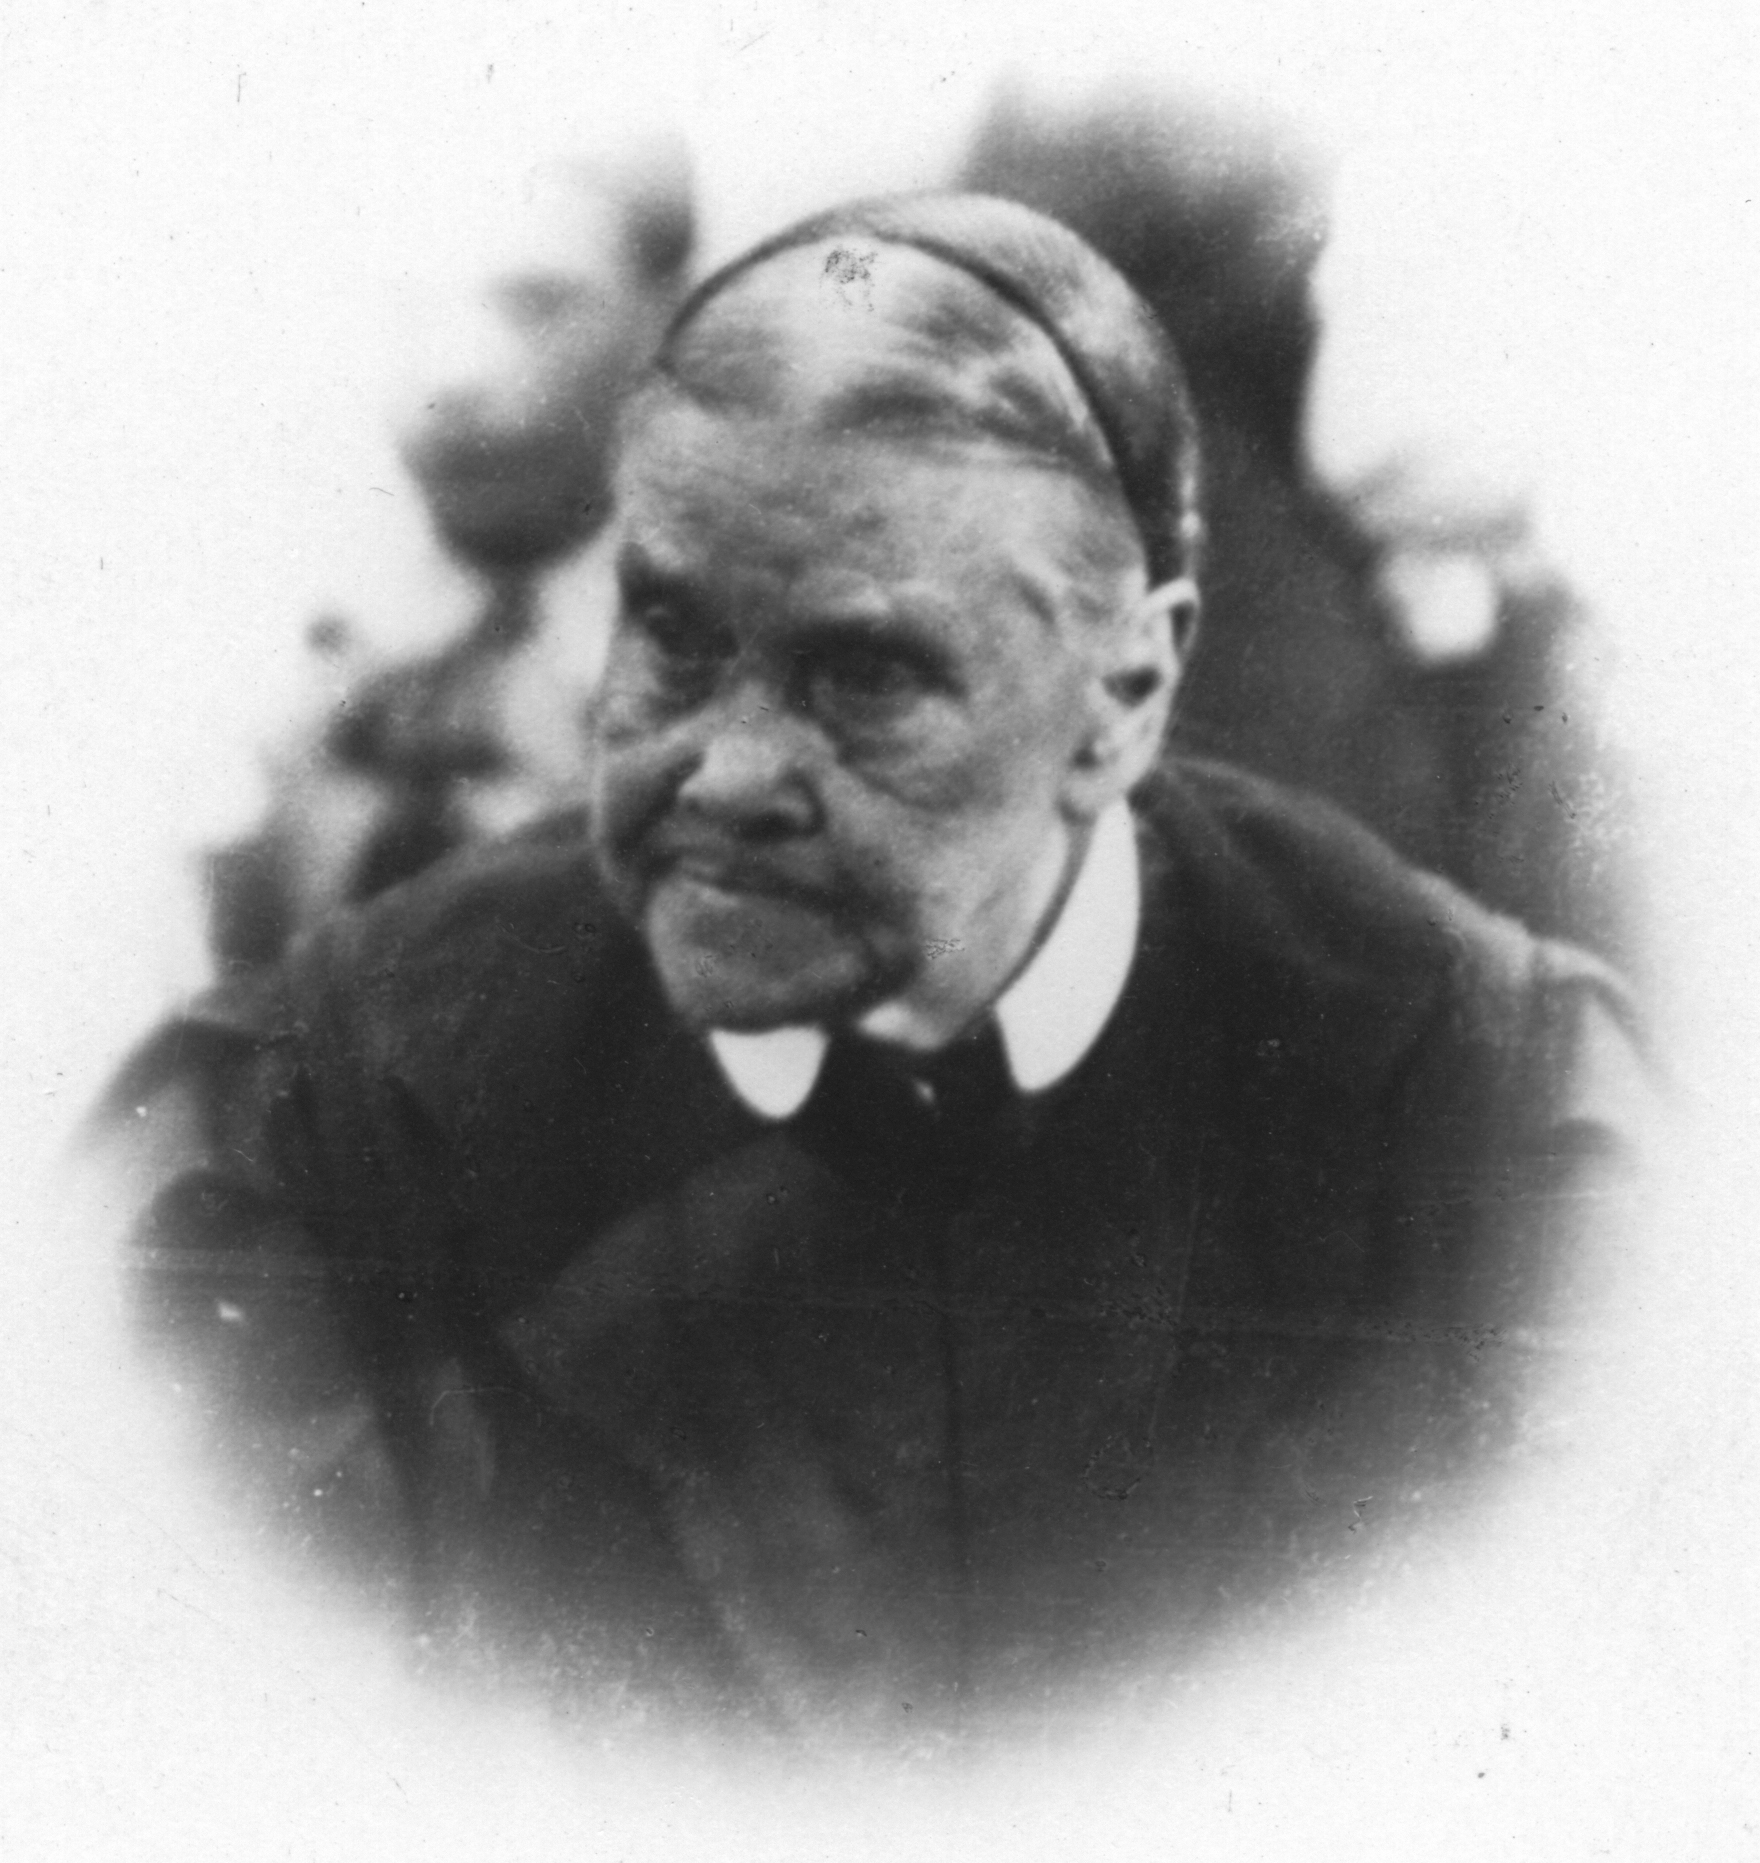
\includegraphics[width=1\linewidth]{images/ellen-white-1913.jpg}
    \caption*{Ellen G. White, 1913}
    \label{fig:e-white-1913}
\end{figure}

Sister White foretold us the future. We watch its fulfilment today. Comparing the \emcap{Fundamental Principles} with today’s Fundamental Beliefs, we see that our religion has changed. Our belief regarding the \emcap{personality of God} has changed. Books of a new order have been written, which are not based on the solid Word of God. A system of intellectual philosophy has been introduced.

This reformation took place in her time. This is how she described the days of the Seventh-day Adventist Church in her time and in the future:

\egw{The present is a solemn, fearful time for the church. The angels are already girded, awaiting the mandate of God to pour their vials of wrath upon the world. Destroying angels are taking up the work of vengeance, for the Spirit of God is gradually withdrawing from the world. Satan is also mustering his forces of evil, going forth ‘unto the kings of the earth and of the whole world,’ to gather them under his banner, to be trained for ‘the battle of that great day of God Almighty.’ \textbf{Satan is to make most powerful efforts for the mastery in the last great conflict. \underline{Fundamental principles will be brought out, and decisions made in regard to them}. Skepticism is prevailing everywhere}. Ungodliness abounds. \textbf{The faith of individual members of the church will be tested as though there were not another person in the world}...}[Ms1a-1890.8; 1890][https://egwwritings.org/read?panels=p6780.13]

Satan's most powerful efforts are to remove the \emcap{Fundamental Principles} by veiling them in skepticism. Judging from today’s perspective we testify to the truthfulness of Ellen White’s prophecies.

\egw{I tell you now, that when I am laid to rest, \textbf{great changes will take place}.}[Ms1-1915.2; 1915][https://egwwritings.org/read?panels=p10771.9]

The true question we have for ourselves is, when the \emcap{Fundamental Principles} are being brought out, what decision will I make in regard to them? Shall we not repudiate everything that is not in harmony with these principles? What decision will you make?

% The future of the Fundamental Principles

\begin{titledpoem}
    \stanza{
        In the early whisper of prophecy’s sound, \\
        Ellen White warned where dangers abound. \\
        "The enemy plots," she sternly declared, \\
        "To dismantle truths our forebears shared."
    }

    \stanza{
        Fundamental Principles, strong and sure, \\
        Once the bedrock, pure and unpure. \\
        Now the sands shift beneath our creed, \\
        Where new doctrines grow like wayward weed.
    }

    \stanza{
        Reformation masked as light so bright, \\
        Undermines the pillars, eroding right. \\
        Books rewritten, philosophies anew, \\
        Skepticism veils what once we knew.
    }

    \stanza{
        Shall the Sabbath lose its sacred glow? \\
        Shall we forget the God that we owe? \\
        "The foundation crumbles," so it seems, \\
        As truth is lost to intellectual dreams.
    }

    \stanza{
        Look back to the days, to the Spirit-led start, \\
        Where divine truths were etched in heart. \\
        Satan’s strategies, cunning and keen— \\
        Eroding what once was clearly seen.
    }

    \stanza{
        So, brethren, now to the past return, \\
        To the roots of faith, let our hearts yearn. \\
        For the warnings spoken, the visions seen, \\
        Call us to defend what they truly mean.
    }

    \stanza{
        Stand firm in the storm as the tempests roar, \\
        Reclaim the truths worth fighting for. \\
        Ellen’s voice echoes, stark and clear: \\
        "Repudiate the false, hold the righteous near."
    }

    \stanza{
        Make your choice, as the battle lines draw, \\
        On the side of the timeless, divine law. \\
        To the Fundamental Principles, fiercely hold, \\
        The original faith, courageous and bold.
    }
\end{titledpoem}